\section{Current \ac{KAUST} system}
The aim of the system that is being built at \ac{KAUST} is to provide a high
speed point to point \ac{UOWC} link using lasers. The initial system will be
static, but a sophisticated tracking system is being developed to ensure the
lasers stay aligned with each other.

This will then be developed into a multiple node network allowing optimum
topologies, both vertical from the surface and horizontal between underwater
nodes.

The system should be low power so that it can run from a reasonable sized
battery pack attached to the underwater nodes, and should be able to last for
a few hours.

\subsection{Current System}
This section describes the current setup in terms of hardware and software
that has been implemented.

\begin{figure}[H]
  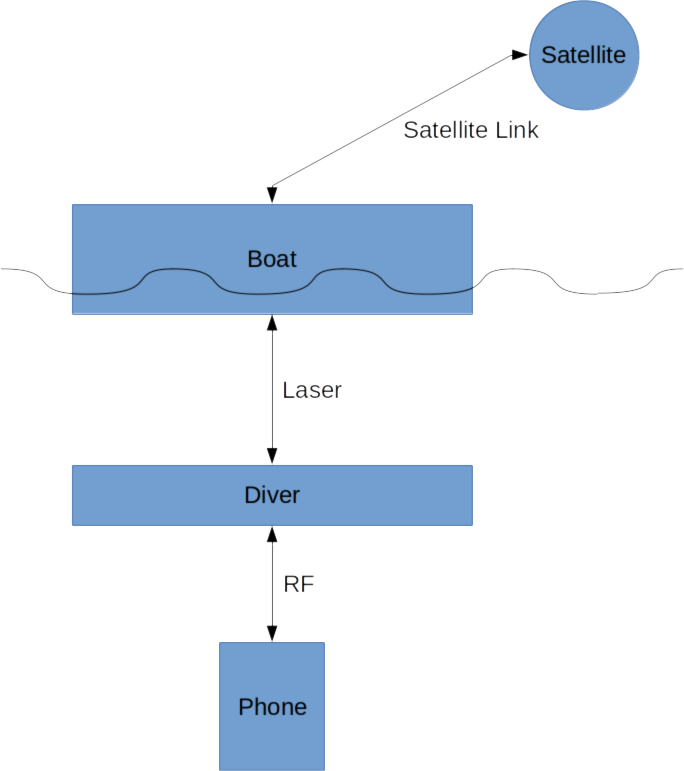
\includegraphics[width=0.8\textwidth]{ship_to_diver.png}
  \caption{Ship to Diver setup}
  \label{fig:ship-to-diver}
\end{figure}

\subsubsection{Hardware}
The current system at \ac{KAUST} is built using a Nichia Green laser (NDG7K75T)
as the transmitter, and a Thorlabs DET10A2 Si Biased Detector for the receiver.

The laser transmitter is connected via a Bias Tee, used to set the DC bias
for the laser to the \ac{UART} TX line of a Raspberry Pi.

The receiver is connected via an amplifier and comparator, to the RX UART
line of the Raspberry Pi.

This is duplicated on both ends of the system, so that a full duplex
system is realized.

\subsubsection{Software}
pppd is used to create an OOK link, using the \ac{UART} link. One Pi is
bridged to the Ethernet interface, allowing a connection to the Internet.
The other Pi (the 'remote') side is bridge to the WiFi interface. A mobile
phone or tablet is then used to connect via WiFi to the Pi. This thus allows
the phone to connect to the Internet.

The bits per second rate of the \ac{UART} is set to 230400. This is pretty fast
for a \ac{UART} interface (only 460800 and 921600) are higher, but for
communications this can only reach 230 Kbp/s (using \ac{OOK}).

Bridging is done by utilising ipv4 forwarding and iptables. This could also
be done by creating a bridge interface and linking the two interfaces together.

dnsmasq is provided at the access point end to automatically assign the phone
an IP address.

systemd is used to start the processes on boot, which is the standard way
of doing system initialisation currently.

\subsection{System Issues}
The current implemented system suffers from a number of limitations. These are
poor performance, lack of \ac{AGC} and no automatic alignment between nodes.

\subsubsection{Poor performance}
The current system is limited to a transmission rate of about 1 Mb/s. The use
of the \ac{UART} is the main limitation in terms of system performance. The baud
rate cannot be pushed very high. In terms of interfaces, the Raspberry Pi has
\ac{SPI}, \ac{I2C} and \ac{UART} connections. None of these are suitable for
a system targeting gigabit performance.

Higher speed interfaces, such as gigabit Ethernet, \ac{SFP}, \ac{PCIe} or
\ac{USB} 3.0 and above, are required. A high speed processor that can process
the data quickly enough is also required.

We should replace the Raspberry Pi with something like
\url{https://mikrotik.com/product/RB922UAGS-5HPacD#fndtn-specifications}

\subsubsection{Lack of \ac{AGC}}
Currently the system must be tuned depending on the range by manually
adjusting the amplifier at the receiver. This system needs refining so that
the adjustments can be made electronically and in real time.

In traditional \ac{AGC} the receiver starts each packet at maximum gain,
which is then reduced as the preamble is received and the signal strength
is measured.

Another approach would be to measure the signal strength out of band and
adjust accordingly. As the laser link is always on, this approach should work.

\subsubsection{No automatic alignment}
The laser beam is very narrow. It is very difficult to align the two ends
to ensure consistent system performance. Both sides must track the other in
order to adjust their beams accordingly.

Beam alignment can be done in-band or out-of-band. In out-of-band, a different
control mechanism is used to localize and track each station. There are two
that are being thought about at the moment, the first being acoustic (which
has been done previously) and the second using cameras to visually track the
laser beam.

An in-band system would use the laser link itself and measure the \ac{SNR} or
\ac{RSSI} values received whilst moving the laser slightly, to ensure the best
angle is chosen.

If an in-band system is required, this must be factored in to the protocols
used as time is required to utilize the lasers for measurements. This must
be designed in from the outset and thus a system that understands beam forming
and movable stations must be used. For example, an 802.11-based \ac{MAC} could
be used, where the protocol allows for scanning time between nodes.

\subsubsection{Low Power}
The system must be low power in order to function underwater with the limited
amount of room available to mount batteries. There does not appear to have been
any testing of the laser in terms of how much power it will draw. Processors
and systems must also be low power, but able to perform appropriately for
the data rates required.
